%
%  Example Appendix pages.
%  Modified to use new usu-thesis-mk2 appendix facilities.
%
%  Time-stamp: "[appendix.tex] last modified by Scott Budge (scott) on
%  2021-06-28 (Monday, 28 June 2021) at 09:03:44 on goga.ece.usu.edu"
%
%  Info: $Id: appendix.tex 1183 2021-06-28 16:49:30Z scott $   USU
%  Revision: $Rev: 1183 $
% $LastChangedDate: 2021-06-28 10:49:30 -0600 (Mon, 28 Jun 2021) $
% $LastChangedBy: scott $
%
%
% For a single appendix, use \makeappendix, and place the 
% body of the appendix after it

%\makeappendix

% < single appendix body here >

% For multiple appendices, use \makeappendices, and create each appendix
% using \appendix{}
% For sub-appendices use \appendixsection{} and \appendixsubsection{}

\makeappendices
\appendix{Voting Distributions}\label{chap:voting-distributions}

\appendixsection{Percent inside Extents}
% TODO: Add description of table
This is placeholder text to ensure
\autoref{tab:distributions-percent-inside-extents} stays in the correct
location. % FIXME

% - Distribution of votes
%     - Uniform
%     - Gaussian
%     - Bimodal about center
%     - Skewed?

\begin{table}[htbp]
    % increase table row spacing, adjust to taste
    \renewcommand{\arraystretch}{1.3}

    \caption{List of distributions used by agents to vote.}
    \label{tab:distributions-percent-inside-extents}

    \centering
    \begin{tabular}{|c|c|c|}
        \hline
        Distribution      & Notation      & Percent inside Extents \\
        \hline
        Uniform           & \uniformdist  & 100\%                  \\
        \hline
        Normal (Gaussian) & \gaussiandist & 99.7\%                 \\
        \hline
        Beta              & \betadist     & 100\%                  \\
        \hline
    \end{tabular}
\end{table}

\appendixsection{Distributions used}
% TODO: Add graphs of distributions used
\begin{table}[htbp]
    % increase table row spacing, adjust to taste
    \renewcommand{\arraystretch}{1.3}

    \caption{List of distributions used by agents to vote.}
    \label{tab:distributions}

    \centering
    \begin{tabular}{|c|c|c|}
    \end{tabular}
\end{table}

\appendixsection{Distributions of Error}
The distribution of square error for each voting mechanism is displayed as a
KDE graph in \autoref{fig:voting_mechanisms_distribution}.

\begin{figure}[!t]
    \centering
    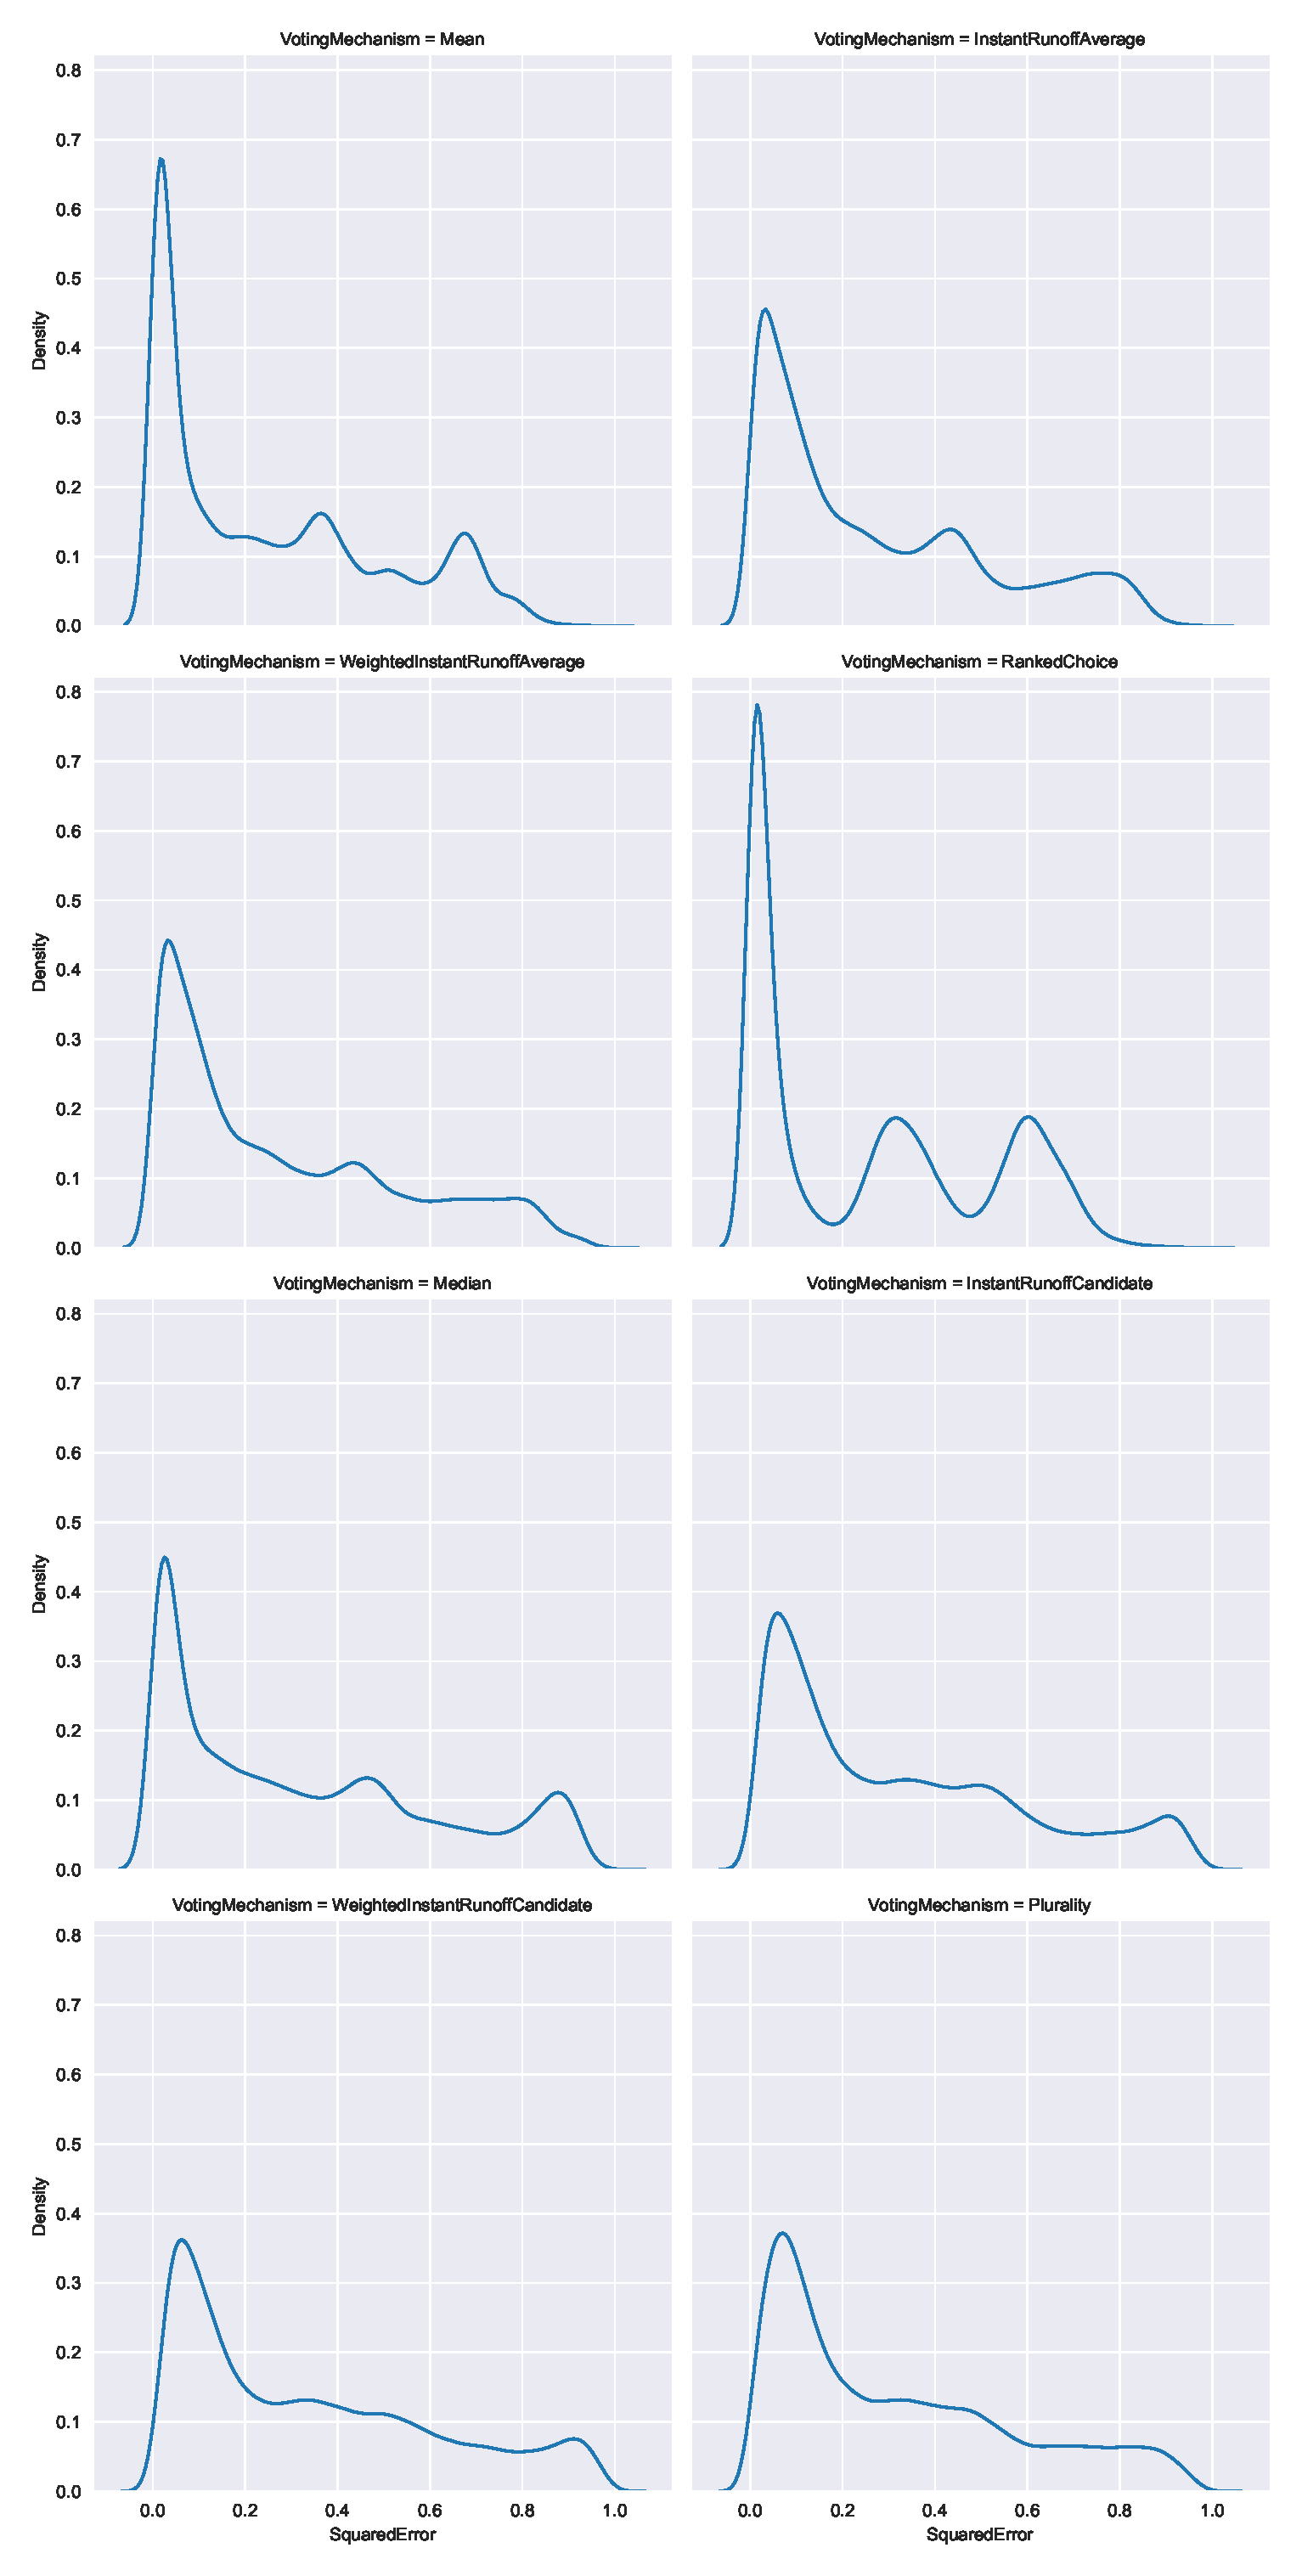
\includegraphics[
        width=\textwidth,
        height=\dimexpr
        \textheight - 2 % Could also be .9\textheight
        \baselineskip,
        keepaspectratio]
    {./content/figures/voting_mechanisms_distribution}
    \caption{The distribution of squared error by voting mechanism}
    \label{fig:voting_mechanisms_distribution}
\end{figure}
